\usepackage{graphicx}\begin{Document}
    Ezt a szoftvert 2024-ben kezdtem el fejleszteni, de a lényegi részét idén készítettem, folyamatos fejlesztéssel, hibajavítással, kísérletezéssel.
    A "keretrendszer", bár én inkább modulnak hívom, 3 fő futtatható állományból áll:
    \begin{itemize}
        \item
    \end{itemize}
    példa válasz a `Qwen/Qwen2.5-0.5B-Instruct` futtatására:
    \begin{figure}
        \centering
        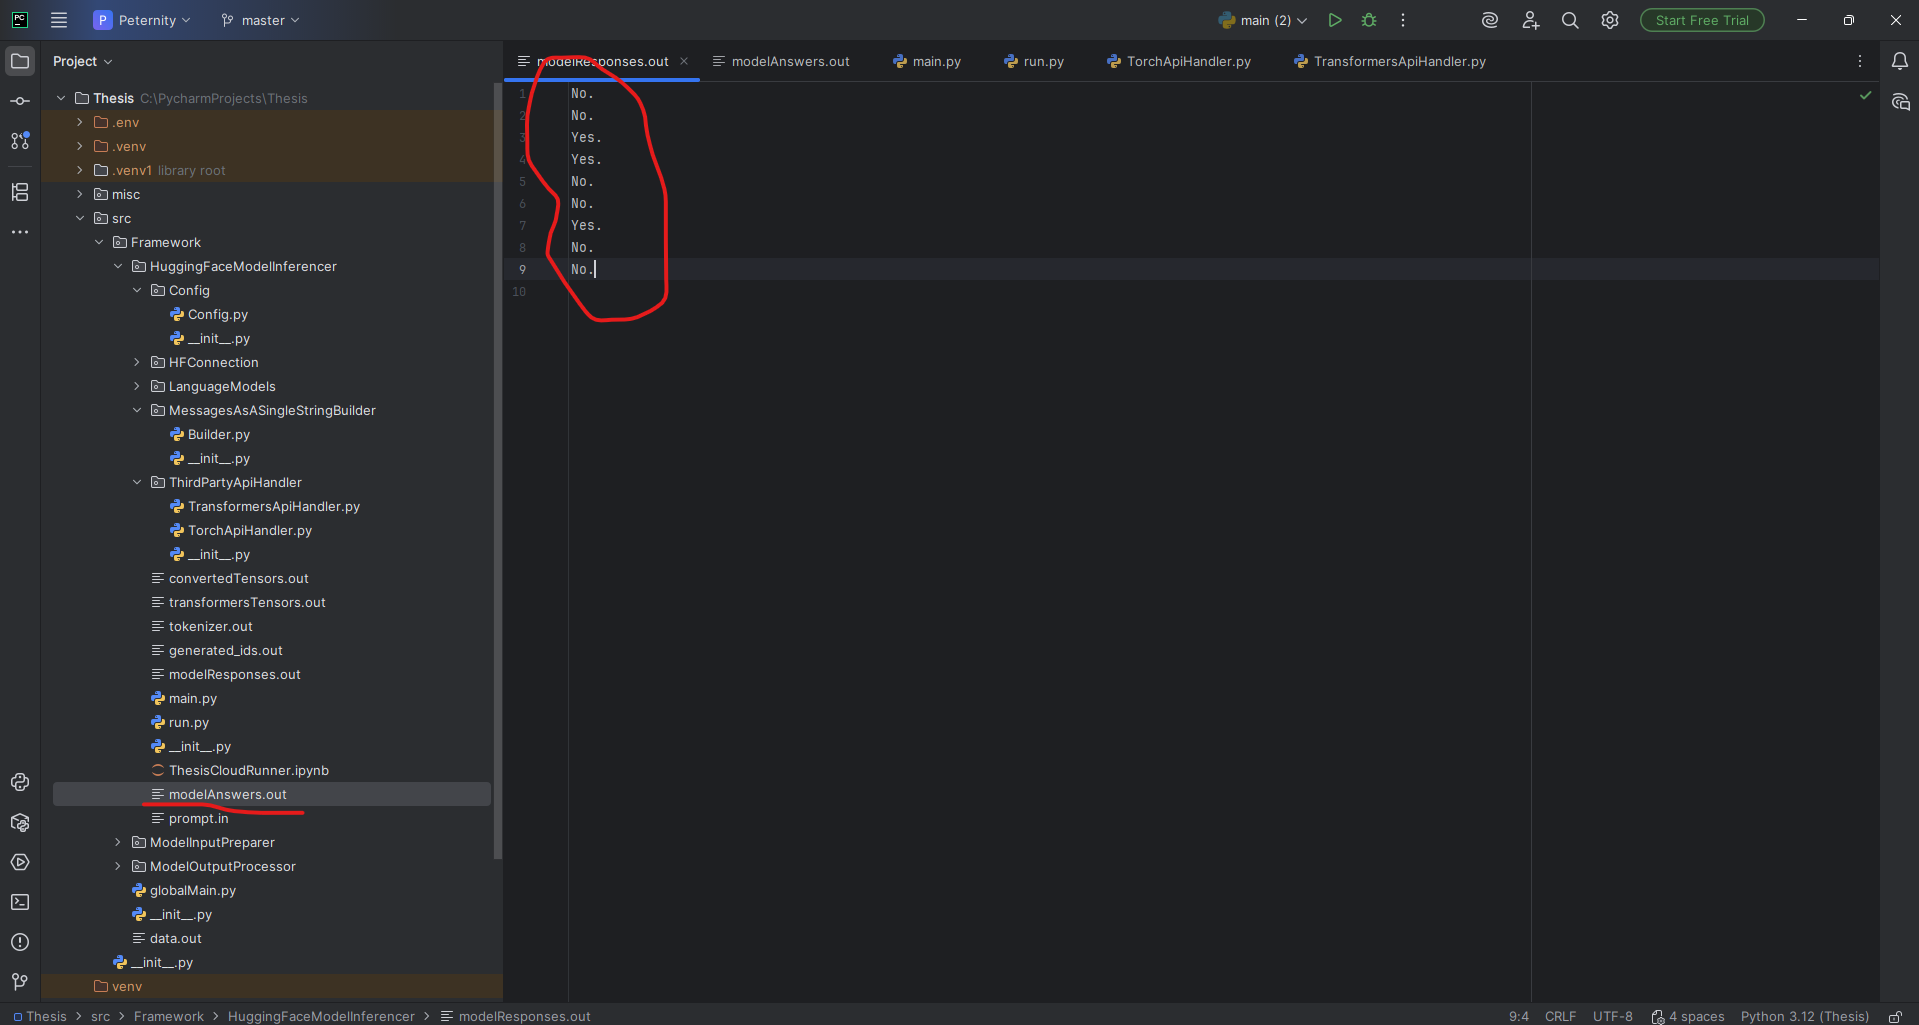
\includegraphics[keepaspectratio]{pelda}
        \caption{Példa Válasz}
        \label{fig:PeldaValasz}
    \end{figure}
\end{Document}